%\clearpage
\section{Introduction}

%\paragraph*{\color{purple}Context}
Most modern software systems can be customized via configuration options to meet user demands. Configuration options can enable desired functionality or tweak non-functional aspects of a software system, such as improving performance or energy consumption. The relationship of configuration choices and their influence on performance has been extensively studied in the literature~~\cite{dorn2020,siegmundPerformanceinfluenceModelsHighly2015,haDeepPerf2019,perfAL,guoVariabilityawarePerformancePrediction2013,sarkarCostEfficientSamplingPerformance,guo_2018_data,fourier_learning_2015,perLasso}. The backbone of performance estimation are prediction models that map a given configuration to the estimated performance value. Learning performance models relies on a training set of configuration-specific performance measurements. In state-of-the-art approaches observations usually employ only a single workload which aims at emulating a specific real-world application scenario.

The choice of the workload (i.e., the input fed to the software system) is known to influence the performance of configurable software systems in different ways as has been shown for the domains of SAT solvers~\cite{falkner_sat_solvers_2015,satzilla_2008}, compilation~\cite{ding_compilation_2015,plotnikov_compilation_2013}, video transcoding~\cite{maxiaguine_workload_2004,alves_sampling_2020}, data compression~\cite{khavari_compression_2019}, and code verification~\cite{koc_satune_2021}. Besides apparent interactions, such as performance scaling with the size of a workload, qualitative aspects can result in more complex and non-trivial performance interactions. For instance, \citeauthor{alves_sampling_2020} have shown that the video transcoder \textsf{x264} exhibits different performance distributions depending on the video source file~\cite{alves_sampling_2020}, and \citeauthor{liao_2020_using_emse} have confirmed this for stream processing applications~\cite{liao_2020_using_emse}. As varying the workload adds another layer of complexity to modeling performance, we cannot guarantee that performance models trained with a single workload \textit{generalize} to arbitrary workloads and make meaningful estimations. 

%\paragraph*{\color{purple}Motivation}
To address this limitation, two different directions have been pursued in the literature. First, performance models trained using a specific workload can be adapted to another specific workload~\cite{jamishidi_transfer_2017,jamshidi_learning_2018,jamshidi_transfer_gp_2017}. Second,  one can specify workload characteristics as further independent variables when modeling configuration-dependent performance~\cite{koc_satune_2021}.
The first strategy direction relies on transfer learning techniques, where, given an existing performance model, in a separate step only the differences to a new environment are learned. Such a transfer function encodes which configuration options’ influence on performance is sensitive to workload variation. While transfer learning is an effective strategy that is not limited to varying workloads~\cite{jamshidi_learning_2018}, but can also be applied to different versions~\cite{jamishidi_transfer_2017,jamshidi_transfer_gp_2017,martin_transfer_2021}, or hardware setups~\cite{ding_bayesian_2020}, its main limitation is that the transfer function is specific to the differences between two environments.

In contrast to transfer learning, a more generalist approach is to consider the input fed to a software system as a further dimension for modeling performance. Here, a workload can be characterized by properties that---individually or in conjunction with software configuration options---influence performance. For such a strategy to work, one requires knowledge of the characteristics of a workload that influence performance. This strategy has been effectively tested for a  variety of application-domains, such as program verification~\cite{koc_satune_2021}. However, the added complexity comes at significant cost. 
Not only does this require substantially more measurements, we often lack knowledge of which performance-relevant characteristics best describe workloads.
 
%\paragraph*{\color{purple}Problem}
The existing body of research reflects the prevalence and importance of the workload influence on software systems~\cite{khavari_compression_2019,maxiaguine_workload_2004,plotnikov_compilation_2013,ding_compilation_2015,falkner_sat_solvers_2015,satzilla_2008,alves_sampling_2020}. All these works are aware of the workload dimension as a factor of performance variation, yet little is known about the quality and driving factors of the \emph{interplay} between configuration options and workloads. Our understanding of this cross-factor relationship lacks knowledge of the following aspects:

\begin{compactitem}
	\item How different is configuration-specific performance across different workloads? 
	\item How many configuration options are responsible for differences in workload-specific performance behavior?
	\item What are the driving factors of the interplay between configuration options and workloads with regard to performance? 
\end{compactitem}

To answer these questions, we have conducted a systematic empirical study that sheds light on whether and how configuration options and workload choices interact with regard to performance. 
Specifically, we analyze 29\,347 configurations and 55 workloads across six configurable software systems to obtain a broad picture of the interaction of configuration and workload when learning performance models and estimating a configuration's performance (i.e., response time). Aside from studying the sole effects of workload variation on performance behavior, we explore possible driving factors. To this end, we enrich performance observations with corresponding statement coverage data to understand workload variation at finer granularity.

Our findings show that varying the workload can influence con\-fi\-gu\-ra\-tion-de\-pen\-dent software performance in different ways, including non-linear and non-monotonous effects. Our findings suggest that (a) coverage of code  specific to configuration options as well as (b) how such code is utilized are driving factors of input sensitivity. A key insight is that, to maintain and improve performance model representativeness, an additional notion of input sensitivity has to be considered. We argue that the use of code analysis techniques to address input sensitivity when varying the workload and maintain and improve the representativeness of a performance-prediction model.

To summarize, we make the following contributions: 

\begin{compactitem}
	\item An empirical study of 29\,347 configurations and 55 workloads across six configurable software systems on whether interactions of workloads with configuration options affect performance and what factors can drive such interactions;
	
	\item A detailed analysis that illustrates that variation in code coverage and code utilization due to varying workloads can affect the influence of configuration options on software performance; 
	
	\item A companion Web site\footnote{\url{https://github.com/fse-submission-2022/workload-performance/}} with supplementary material including performance and coverage measurements, experiment workloads and configurations, and an interactive dashboard\footnote{\url{https://workload-performance.herokuapp.com/}} for additional visualizations left out due to space limitations.
\end{compactitem}



\begin{comment}
Most software systems can be customized via configuration options to meet user demands. The selection of configuration options can enable desired functionality (features) or tweak non-functional aspects of a software system, such as improving performance or energy consumption. 
The relationship of configuration choices and their influence on performance has been extensively studied in literature.
The backbone of performance estimation is a model that maps a given configuration to the estimated performance value. 
Learning performance models usually relies on a training set of configuration-specific performance measurements. 
To measure performance, established approaches~\cite{dorn2020,siegmundPerformanceinfluenceModelsHighly2015,haDeepPerf2019,perfAL,guoVariabilityawarePerformancePrediction2013,sarkarCostEfficientSamplingPerformance,guo_2018_data,fourier_learning_2015,perLasso} usually employ only a single workload (e.g., a benchmark or test suite), which aims at emulating a specific real-world application scenario.

Conversely, for performance and load testing in practice, workloads are a widely considered as a key factor for performance variation~\cite{ceesay2020,papadopoulos2021}.
In the domain of cloud computing applications~\cite{papadopoulos2021} and data-intense applications~\cite{ceesay2020}, methodological principles emphasize the importance of using representative workloads or testing against a set of workloads that reflect the system under test and account for workload-specific behavior. Methods for finding such representative workloads are known under the umbrella term \emph{workload characterization}~\cite{calzarossa2016} and are widely used alongside mixes of different workloads in practice~\cite{jiang2015survey}. 

Both configuration-dependent and workload-dependent performance behavior have been studied mostly in isolation. While there are some attempts to gain insights on their combination for specific application scenarios~\cite{alves_sampling_2020}, under limited variability~\cite{liao_2020_using_emse}{\color{purple}, and for a specific problem domain~\cite{koc_satune_2021}}, to the best of our knowledge, we are the first to systematically explore the intersection of both factors of variation {\color{purple} across multiple domains}. We aim at providing a clear picture of how prevalent and severe workload-specific differences in configuration-dependent performance are and how they emerge in the wild. 
To illustrate, how both factors may interact, consider the introductory example of an imaginary database system in Figure~\ref{fig:intro}. The method in this example handles an array of insertions. The workload determines how configuration-dependent code is utilized, such as the execution of \colorbox{duplicatecheck}{Lines 2--6} for configuration option \texttt{DUPLICATE\_CHECK}. A performance model that considers this dependency as an input factor might be more representative than a performance model that was trained on a single workload. If a workload, however, conditions the execution of configuration-specific source code, such as \colorbox{autocommit}{Lines 12--14} for configuration option \texttt{AUTOCOMMIT}, one can derive a more representative performance modes from selecting workloads that increase overall code coverage, similar to test coverage.

%In absence of a systematic study that sheds light on whether and how configuration options and workload choices interact with regard to performance, we address this isssue in this paper. 
We have conducted an empirical study of 29\,014 configurations and 55 workloads across 6 configurable software systems to provide a broad picture of the interaction of configuration and workload when learning performance models and estimating a configuration's performance (i.e., response time). Aside from studying the sole effects of workload variation on performance behavior and performance model influences, we explore \emph{how} both factors interact. To this end, we enrich performance observations with corresponding statement coverage data to understand workload variation at a finer grain. This way, we reveal whether workload-specific effects can be attributed to specific code segments or rather depend on workload-specific code usage.

Our findings suggest that the workload-specific
execution of covered option-specific code segments plays a substantial role in how workloads interact with configurations and is most likely accountable for workload-specific performance variation. We conclude that identifying performance-relevant workload characteristics and incorporating them as independent variables is
a promising avenue towards obtaining generalizable and representative performance models.

To summarize, we make the following contributions: 
	
\begin{compactitem}
	\item An empirical study of 29\,014 configurations and 55 workloads across 6 configurable software systems of whether and how the interaction of workloads with configuration options influences performance;
	
	\item An evaluation combining insights from observations of workload-specific differences of configurations, individual configuration options' influence on performance, and workload-specific coverage differences of option-specific code segments;

	\item A companion Web site\footnote{\url{https://github.com/anonyms-2021/submission-448/}} with supplementary material including performance and coverage measurements, experiment workloads and configurations, as well as additional visualizations left out due to space limitations.
\end{compactitem}
\end{comment}


\section{Background and Motivation}
\subsection{Performance Prediction Models}~\label{sec:perfmodels}
Configurable software systems are an umbrella term for any kind of software system that exhibits configuration options to customize functionality. 
While the primary purpose of configuration options is often to select and tune functionality, each configuration choice may also have implications on non-functional properties --- be it intentional or unintentional. Finding configurations with optimal performance~\cite{nairUsingBadLearners2017,nairFlash18,ohFindingNearoptimalConfigurations2017} and estimating the performance for arbitrary configurations of the configuration space is an established line of research~\cite{siegmundPerformanceinfluenceModelsHighly2015,haDeepPerf2019,perfAL,guoVariabilityawarePerformancePrediction2013,sarkarCostEfficientSamplingPerformance,guo_2018_data,fourier_learning_2015,perLasso}. 
Machine-learning techniques have been used to learn \emph{performance models} that approximate non-functional properties, such as execution time or memory usage, as a function of software configurations $c \in C$, formally $\Pi: C \rightarrow \mathbb{R}$.

Performance models can be obtained using a variety of machine-learning techniques, including probabilistic programming~\cite{dorn2020}, multiple linear regression~\cite{siegmundPerformanceinfluenceModelsHighly2015}, classification and regression trees~\cite{sarkarCostEfficientSamplingPerformance,guo_2018_data}, Fourier learning~\cite{fourier_learning_2015,perLasso}, and deep neural networks~\cite{haDeepPerf2019,perfAL}.
The set of configurations for training can be sampled from the configuration space using a variety of different sampling techniques. All sampling strategies aim at yielding a representative sample, either by covering the main effects of configuration options and interactions among them~\cite{siegmundPredictingPerformanceAutomated2012}, or sampling uniformly from the configuration space~\cite{ohFindingNearoptimalConfigurations2017,kaltenecker_distance-based_2019}.
Most approaches share the perspective of treating a configurable software system as a black-box model at application-level granularity. Recent work has incorporated feature location techniques to guide sampling effort towards relevant configuration options~\cite{velez_2020_configcrusher_jase,velez_comprex_2021} or model non-functional properties at finer granularity~\cite{weber_white_2021}.

\subsection{Varying Workloads}
\subsubsection{Whats is a workload?}
For the following, we conceive a workload as any form of \textit{input fed to a software system for processing}. By nature, the workload of a software system is application-specific, such as a set of queries and transactions fed to a database system, a set of raw image files for video encoding, or an arbitrary file for data compression etc. Each workload $w \in W$, similarly to configurable software systems, exhibits characteristics (or dimensions) that can be used to describe and quantify its properties.

\subsubsection{Workload Characterization}\label{sec:workload-characterization}
In performance engineering, workload characterization is a well-defined and widely employed task~\cite{} in order to reason about the performance of a software system and systematically assess software quality across a diverse set of workloads. 
It is common practice to select a workload that is reflective of the software system in question~\cite{ceesay2020,papadopoulos2021}. This can be achieved by constructing workloads, among others, from usage patterns~\cite{calzarossa2016}, or by increasing the workload coverage by using a mix of different workloads rather than a single one~\cite{jiang2015survey}.\todo{hier könnte noch mehr hin... siehe analytical models oder CPU vs. memory bound workloads. man könnte auch noch etwas zu community benchmarks schreiben, wie SPEC, TPC, etc.}

%However, one cannot guarantee that it yields the complete set of characteristics and therefor knowledge of the domain of possible workloads. Some characteristics can be non-trivial in that they might not be documented or known to developer, or only become relevant for performance under a specific configuration of a software system. Thus, from workload characterization, at best, one can assume an approximation of the workload domain model.


\subsection{Input Sensitivity Limits Generalizability}\label{sec:generalizability}
A major threat to the practicality of approaches outlined in Section~\ref{sec:perfmodels} lies in their use of only a \textit{single} workload. A model is trained on performance data gained by of varying configurations while keeping the workload the same. Clearly, this can limit the model’s generalizability to different workloads. While the configuration-specific behavior might be congruent across some workload, i.e, the best-performing configuration for one workload may also be the best-performing for another one, we cannot rely on such assumptions in practice, where different workloads can result in entirely different configuration-specific performance behavior~\cite{alves_sampling_2020}.

Revisiting an observation by \citeauthor{alves_sampling_2020}, the following example illustrates that even seemingly small differences in the composition of a workload can induce performance behavior that is hard to anticipate: We tested the performance (throughput: transactions per second) of a number of configurations for the database system \htwo across two different workloads. Both workloads are a parameterization of the database benchmark \textsf{TPC-C}, consisting of a fixed-ratio mix of transactions (inserts, updates, selects) for a specific database schema. The only difference was varying the scale factor, which controls for the number of warehouses modeled in the schema. The resulting performance distributions for both experiments are illustrated in Figure~\ref{fig:h2_intro}.

\begin{figure}
	\centering
	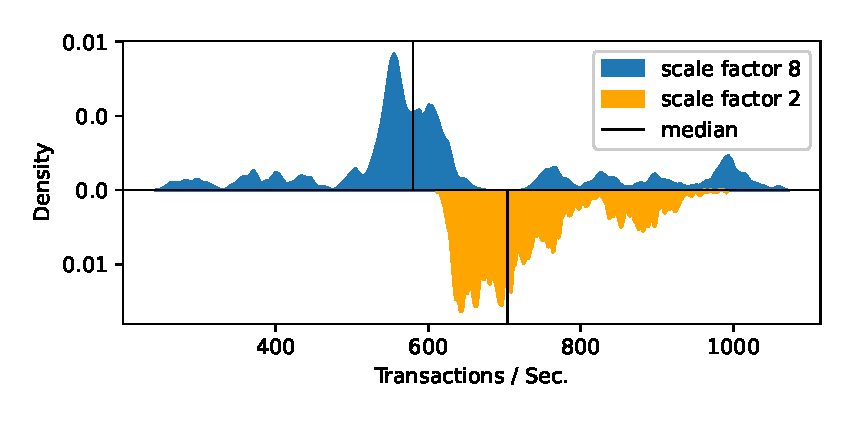
\includegraphics[width=0.9\linewidth]{images/h2_motivation.eps}
	\caption{Performance distributions of \htwo and the \textsf{TPC-C} benchmark at different scale factors.}
	\label{fig:h2_intro}
\end{figure}

While one might first expect that a more complex workload results in lower throughput, this is correct, but does not hold for all configurations. We see that the median throughput indeed decreases when increasing the scale factor, however the \emph{shape} and the \emph{spread} of the performance distribution is affected as well, which cannot be expect when all configurations scale evenly. The majority of configurations’ performance scales with the workload, some do not and even few achieve improved throughput. Thus, if configurations’ performance is affected in such non-trivial ways, varying the workload affects the performance influence that different configuration options exhibit. 

Some aspects of this \emph{input sensitivity} has been observed and documented before in the literature~\cite{liao_2020_using_emse,alves_sampling_2020,jamishidi_transfer_2017} and raise questions, such as: Which options are input sensitive? What workload characteristics affect an option’s performance-influence? Can we estimate which options are input-sensitive? We set out to answer these questions in this paper.
	
\subsection{Strategies for Handling Varying Workloads} ~\label{sec:strategies}
Research and industry practices can provide answers to some aspects of the three questions from Section~\ref{sec:generalizability}.

\subsubsection{Workload-aware Performance Modeling}\label{sec:workload-aware}
Extending on workload characterization (cf. Section~\ref{sec:workload-characterization}), a strategy that embraces workload diversity is to incorporate workload characteristics into the problem space of a performance prediction model. Here, performance is modeled as a function of both the configuration options exhibited by the software system as well as the workload characteristics, formally $\Pi: C \times W \rightarrow \mathbb{R}$.
The combined problem space enables learning performance models that generalize to workloads that exhibit characteristics denoted by $W$ since we can screen for performance-relevant combinations of options and workload characteristics. Although this strategy is highly application-specific, it has been successfully applied to different domains, such as program verification~\cite{koc_satune_2021} and {\color{red}\cite{}}\todo{references}. However, its main disadvantages are twofold: The inflated and more complex problem space implies substantially more observations to screen for identifying performance-relevant options, characteristics, and combinations thereof. In addition, previous work on exploring the differences across workload-specific performance found that only few configuration options are input sensitive~\cite{jamishidi_transfer_2017}, which exacerbates the problem of finding the meaningful, but sparse predictors.

\subsubsection{Transfer Learning for Performance Models}\label{sec:transfer}
Another strategy that builds upon the fact that, across different workloads, only few configuration options are in fact input sensitive~\cite{jamishidi_transfer_2017}, is to train a model on a standard workload and then adapt it to different workloads. Contrary to a generalizable workload-aware model, transfer learning strategies focus on approximating a transfer function that, without characterizing the workload, encodes the information of which configuration options are sensitive to differences between a source and target pair of workloads. Training a workload-specific model and adapting it on occasion provides an effective means to reuse performance models, which is not limited to workloads~\cite{jamshidi_learning_2018}, but has successfully been applied to different hardware setups~\cite{ding_bayesian_2020} and across versions~\cite{martin_transfer_2021}. 


\subsection{Research Goal}
{\color{red} Neu machen}

The remainder of this paper is organized as follows. In the following Section~\ref{sec:study}, we present our case study and methodology. Section~\ref{sec:results} presents the study results, Section~\ref{sec:categories} presents our findings on categorizing types of input sensitivity. We discuss implications for industry and research in Section~\ref{sec:discussion}, review related in Section~\ref{sec:related} and summarize our findings in Section~\ref{sec:conclusion}.

\section{Study Design}~\label{sec:study}
We have conducted an empirical study of a multitude of configurations and workloads for six configurable software systems. In the following, we describe the general experiment setup and study design as well as research questions and results. We make all performance measurement data, configurations, workloads, and learned performance models available on this paper's companion Web site.

\subsection{Research Questions}
The first two research questions shed light on the input sensitivity of the performance behavior of the studied software systems. We first take a look at systems as a whole~(\RQref{1}) with regard to a large set of configurations and, subsequently, consider individual configuration options~(\RQref{2}). Extending on the results of \RQref{2}, we explore possible driving factors and indicators for workload-specific performance variation~(\RQref{3}).

\subsubsection{Performance Behavior Across Workloads}
It is well known that performance variation can arise from differences in the workload~\cite{benchmarking_book}. In a practical setting, the question arises whether, and if so, to what extent an existing workload-specific performance model is representative of the performance behavior of other workloads as well. 
That is, can a model estimating performance of different configurations be reused for the same software system, but learned under a different workload? Depending on the degree of similarity of the performance behavior across workloads, we can obtain a clearer picture of the prevalence of input sensitivity and to what degree the strategies outlined in  Section~\ref{sec:strategies} might be applicable.
To provide some context for the feasibility of model reuse or transformation, we formulate the following research question: 

\RQ{1}{To what extent does \textit{performance behavior} vary across workloads?}

\subsubsection{Option Influence Across Workloads}
At large, performance behavior is the resulting effect arising from multiple configuration options’ and combinations’ respective influences. To further understand, which configuration options are driving performance variation in general, and are input sensitive in particular, we want to obtain a clearer picture. To this end, we ask the following research question:

\RQ{2}{To what extent do \textit{influences of individual configuration options} depend on the workload?}

\subsubsection{Possible Causes of Input Sensitivity}
To start to translate our findings of performance variation under varying workloads from \RQref{1} and \RQref{2} into actionable strategies, we require insights about how the workload interacts with configuration options. At code level, we outline two possible scenarios: First, option-specific is only covered under a specific workload, so that we can observe its only influence under that workload. 

\RQ{3}{To what extent do influences of configuration options on performance and option-specific code coverage depend on the workload?}

\subsection{Methodology}
\subsubsection{Overview}

\begin{compactenum}
	\item 
\end{compactenum}

\subsection{Experiment Setup}\label{sec:setup}
\subsubsection{Subject Systems}
For our study, we select six configurable software systems implemented in Java. We decided to use Java for mainly two reasons: (1) practically, because we can forgo code modifications for instrumentation by using off-line instrumentation (cf.~Section~\ref{sec:profiling}) for code coverage measurement, and (2) strategically, because Java is one of the most widely used programming languages. We discuss this decision in more detail in Section~\ref{sec:threats}. 
\jumper is a re-implementation of the LAME audio codec for MP3 in Java. \kanzi is a command-line file compression tool. \dconvert is a Java utility to scale images for use in Android apps into different formats and different resolutions. \batik is a Java utility to rasterize vector graphics. \jadx is a decompiler and deobfuscator for Android applications. The full list of our subject systems and characteristics is presented in Table~\ref{tab:subject_systems}. 
For all software systems, we have measured more than one performance metric, except for \htwo, where we measured the throughput.  In the following, we focus on response time and throughput to keep our analysis and results comparable.

\begin{table}[h]
	\footnotesize
	\centering
	\caption{Subject System Characteristics}
	\begin{tabularx}{\linewidth}{lllrrrr}
		\toprule
		\textbf{Software System} &  \textbf{Application Type} & \textbf{Revision} & \textbf{ \#\,O} & \textbf{\#\,C} & \textbf{\#\,W}  \\
		\midrule
		\jumper & Audio encoder & 1.0.4 & 19 & 4\,196 & 6   \\
		
		\kanzi & File compressor & 1.9 & 24 & 4\,112 & 9 \\
			
		\dconvert & Image scaling & 1.0.0-alpha7 & 17 & 6\,764 & 12  \\
				
		\htwo & Embedded database & 1.4.200 & 16 & 1\,954  & 8  \\
		
		\batik & SVG rasterizer & 1.14 & 10 & 1\,919 &  11  \\
		
		\jadx & Java decompiler & 1.2.0 & 18 & 10\,502 & 9  \\
\bottomrule

\end{tabularx}\\
{\vspace{1mm}\textit{Abbreviations: \#\,O: No. of options, \#\,C: No. of configurations, \#\,W: No of. workloads}}

	\label{tab:subject_systems}
\end{table}

\subsubsection{Workload Selection}
We aim at covering a variety of workload characteristics to make use of different functionality of a subject system. 
For the selection of workloads, we considered general characteristics (e.g., workload size to probe for scaling and utilization factors) and domains-specific characteristics that reflect the specific application domain (e.g., different valid input file types).
Due to space limitations, we provide a more extensive description of the used workloads at the paper's companion Web site.

For \jumper, we selected WAVE audio files that, among others, vary in the sampling rate, number of channels, and file size. For \kanzi, we selected dedicated compression benchmark corpora (sets of files of different types) into our selection and further included files of different types at different scales, among others, a binary of the linux kernel and CSV data. For \dconvert, we selected files that reflect the application’s documented input formats (JPEG, PNG, PSD, and SVG) and vary in file size. For \batik, we selected a range of SVG file varying in size. For \jadx, we selected a number popular of Android applications (APK packages) ranging from social media to games and utility applications. For \htwo, we used a selection of application-level benchmarks from \textsc{OLTPBench}~\cite{difallah_oltp_2013}, a load generator for databases that allows for using a variety of performance testing benchmarks, such as \texttt{TPC-C}. 

\subsubsection{Configuration Sampling}\label{sec:sampling}
For each subject system, we sampled a set of configurations. Exhaustive coverage of the configuration space is infeasible due to combinatorial explosion~\cite{henardCombining2015}. We combine several coverage-based sampling strategies and uniform random sampling into an \emph{ensemble} approach: 
To study the influence of single configuration options, we employ option-wise and negative option-wise sampling~\cite{siegmundPerformanceinfluenceModelsHighly2015}, where each option is enabled once, or all except one, respectively. In the same way, pair-wise sampling applies this schema to study influences of two-way interactions between configuration options. Interactions of higher degree can be found accordingly, which, however, is computationally prohibitively expensive~\cite{henardCombining2015}. Instead, we augment our sample set with a random sample that is, at least, twice the size of the coverage-based sample. To achieve a uniform random sample, we used \emph{distance-based sampling}~\cite{kaltenecker_distance-based_2019}. The variability models, as well as sample sets, can be found on the paper's companion Web site.
	
\subsubsection{Coverage Profiling}\label{sec:profiling}
To measure code coverage, we use the on-the-fly profiler \textsc{JaCoCo}. Unlike profilers that use source code instrumentation, with on-the-fly instrumentation, the executable binary remains unchanged. This way, we avoid altering and re-compiling the source code or injecting instrumentation code post compilation. From a practical perspective, on-the-fly instrumentation is more flexible and easier to accommodate. Nonetheless, either choice introduces some performance overhead. To avoid this overhead distorting our performance measurements, we conducted our coverage analysis in a separate run, for which no performance data was collected. 	
	
\subsubsection{Hardware Setup}
All experiments were conducted on three different compute clusters and each subject system was exclusively run on a single cluster. All machines in a compute cluster had the identical hardware setup: either with Intel~Core~i5-8259U CPUs at 2.3~GHz (\jumper and \kanzi),  Intel~Core~i7-8559U CPUs at 2.7~GHz (\dconvert, \batik, and \jadx) and 32~GB of RAM, respectively, or Intel~Xeon~E5-2630~v4 CPUs at 2.2~GHz with 256~GB of RAM (\htwo). All clusters ran a headless Debian 10 installation, the first two with kernel version \mbox{\texttt{4.19.0-14}}, the latter with version \mbox{\texttt{4.19.0-17}}. 
To minimize measurement noise, no additional user processes were running in the background, and no other than necessary packages were installed.	For all data points, we report the median across five repetitions (except for \htwo), which has shown to be a good trade-off between variance and measurement effort. For \htwo, we omitted the repetitions as in a pre-study, running on the identical cluster setup, we found that across all benchmarks the throughput coefficient of variation (standard deviation divided by the arithmetic mean) was consistently below~5\,\%.

\section{Study Results}~\label{sec:results}
\subsection{Comparing Performance Distributions}\label{sec:rq1}
\subsubsection{Operationalization}
We approach \RQref{1} by pairwisely comparing the performance distributions from different workloads (cf. the comparison in Figure~\ref{fig:h2_intro}) and investigate whether any two distributions are similar or, if not, can be transformed into each other. For the latter case, we are specifically interested in what type of transformation is necessary as this determines \textit{how} complex a workload interacts with configuration options. We categorize each pair of workloads with respect to the following aspects: 

\begin{compactenum}
	\item \textbf{Similarity}: As a sanity check, we first ask whether two performance distributions are equal. Such distributions are ususally multi-modal and/or long-tailed~\cite{curtsinger_stabilizer_2013,maricq2018taming}, which fails to meet the requirements for existing parametric siginificance tests. Instead, we employ the Wilcoxon signed-rank test~\cite{lovric_international_2010} to assess whether varying the workload affects configuration performance. If we can reject the null hypothesis $H_0$ at significance level $\alpha~=~0.95$, we consider the distributions dissimilar. In addition, to account for account for overpowering due high and different sample sizes (cf.~Table~\ref{tab:subject_systems}), we report effect sizes to asses whether the effect attributed to varying the workload is negligible or not. We use Vargha and Delaney's $A$ measure~\cite{vargha_delaney_2000} and their proposed threshold of {\color{red}$A \geq 0.7$}, indicating a large effect.
	
	\item \textbf{Linear Correlation}: If both performance distirbutions shifted by a constant value or scaled by a constant factor. To test for this case, we compute for each pair of distributions Pearson's $r$ correlation coefficient. To discard the sign of relationship, we use the absolute value, henceforth $r^*$ and follow {\color{red}Someone's rule} for interpretation, where $\color{red}r^* >0.6$ indicates a strong linear relationship, one can employ a linear transformation. 
	\item \textbf{Monotonous Correlation}: Similarly to the previous aspect and last, we test whether there exists a monotonous relationship between the two performance distributions. We use Kendall's $\tau$~\cite{kendall1938new} rank correlation coefficient and follow {\color{red}Evan's} rule for interpretation, where $\color{red}\tau > 0.7$ indicates a strong monotonous relationship.
\end{compactenum}

{\color{black} Based on these three tests and metrics, we composed four categories, which each pair of performance distributions can be categorized into. If we cannot reject $H_0$, we consider them identical and as similar distributions (\textsf{\colorbox{cs-color}{SD}}). If both distributions exhibit a strong linear relationship, we classify them as linearly transformable (\textsf{\colorbox{lt-color}{LT}}). If we observe a strong monotonous, but not a linear relationship, we classify such pairs as exclusively monotonously transformable into a separate category (\textsf{\colorbox{xmt-color}{XMT}}). Last, if the comparison yields no monotonous relationship, we can only transform them using non-monotonous methods (\textsf{\colorbox{nmt-color}{NMT}}). We summarize the category criteria as well as the category counts in Table~\ref{tab:categorization}. 

\begin{table}[h!]
	\footnotesize
	\caption{Categorization and category counts of configuration-specific performance distributions across workload pairs}
	\centering
\begin{tabular*}{\linewidth}{lp{4.4cm}p{3cm}}	
	\toprule
	 \textbf{Abbrev.} & \textbf{Category} & \textbf{Criteria}\\
	 \midrule
	 \cellcolor{cs-color}\textsf{SD} & {Similar distributions} & {$H_0$ not rejected} \\
	 \cellcolor{lt-color}\textsf{LT} & {Linear transformation} & $r^* \geq 0.6$ \\
	\cellcolor{xmt-color}\textsf{XMT} & {Non-linear, but monotonous transformation} & $r^* < 0.6 $ and $ \tau^* \geq 0.6$ \\
	\cellcolor{nmt-color}\textsf{NMT} & {Non-monotonous transformation}  & (otherwise) \\%$p < 0.05$ and $\tau < 0.6$ \\
	\bottomrule
\end{tabular*}\\
\begin{tabular}{lrrrrrrrr}	
	\toprule
	\textbf{Subject System} & \multicolumn{2}{c}{\textbf{\textsf{SD} Pairs}} & \multicolumn{2}{c}{\textbf{\textsf{LT} Pairs}} & \multicolumn{2}{c}{\textbf{\textsf{XMT} Pairs}} & \multicolumn{2}{c}{\textbf{\textsf{NMT} Pairs}}\\
	 & \textit{abs.} & \textit{rel.} & \textit{abs.} &\textit{ rel.} & \textit{abs.} & \textit{rel.}& \textit{abs.} & \textit{rel.}\\
	\midrule
	\jumper & 1 & 42\,\% & 1 & 42\,\% & 1 & 42\,\% & 1 & 42\,\%\\
	\kanzi & 1 & 42\,\% & 1 & 42\,\% & 1 & 42\,\% & 1 & 42\,\%\\
	\dconvert & 1 & 42\,\% & 1 & 42\,\% & 1 & 42\,\% & 1 & 42\,\%\\
	\htwo & 1 & 42\,\% & 1 & 42\,\% & 1 & 42\,\% & 1 & 42\,\%\\
	\batik & 1 & 42\,\% & 1 & 42\,\% & 1 & 42\,\% & 1 & 42\,\%\\
	\jadx & 1 & 42.5\,\% & 1 & 42.9\,\% & \cellcolor{olive!25!white}1 & \cellcolor{indigo!18!white}90.1\,\% & 1 & 42\,\%\\
	\bottomrule
\end{tabular}
\label{tab:categorization}
\end{table}

\subsubsection{Results}  Results are summarized in the lower part of  Table~\ref{tab:categorization}
{\color{black!40!white}\blindtext}
\vspace{2mm}
\greybox{\textbf{Summary} (\RQref{1}): \ldots}

\subsection{Input Sensitivity of Options}\label{sec:rq2}

\subsubsection{Operationalization}
{\color{red} Linear Regression as Sensitivity Analysis}
{\color{black!40!white}\blindtext}
\subsubsection{Results}
Results are summarized in Figure~\ref{fig:results_influence}
\begin{figure*}
	\centering
	\begin{subfigure}{0.49\textwidth}
		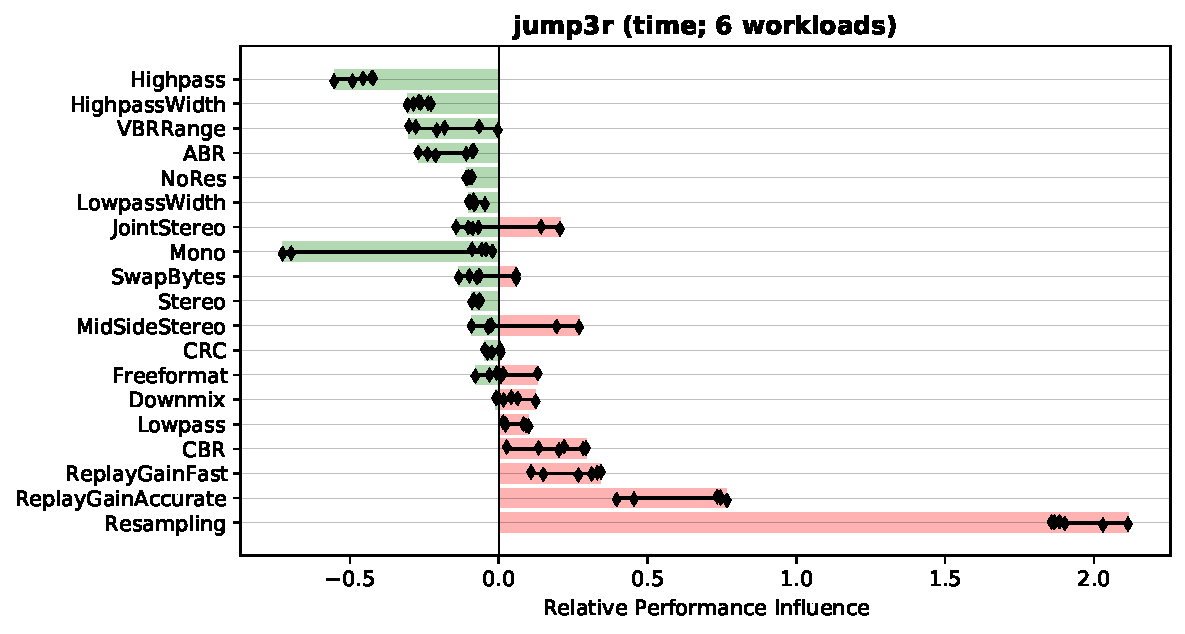
\includegraphics[width=\linewidth]{fse_22/jump3r_rq2.pdf}
	\end{subfigure}
	\begin{subfigure}{0.5\textwidth}
		\centering
		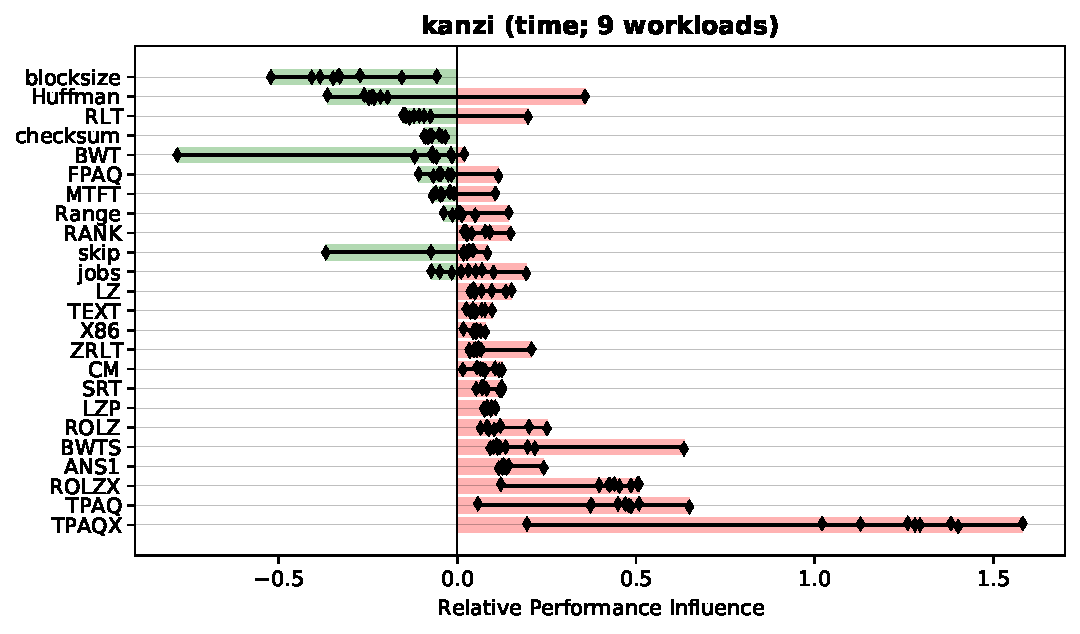
\includegraphics[width=\linewidth]{fse_22/kanzi_rq2.pdf}
	\end{subfigure}

	\begin{subfigure}{0.49\textwidth}
		\centering
		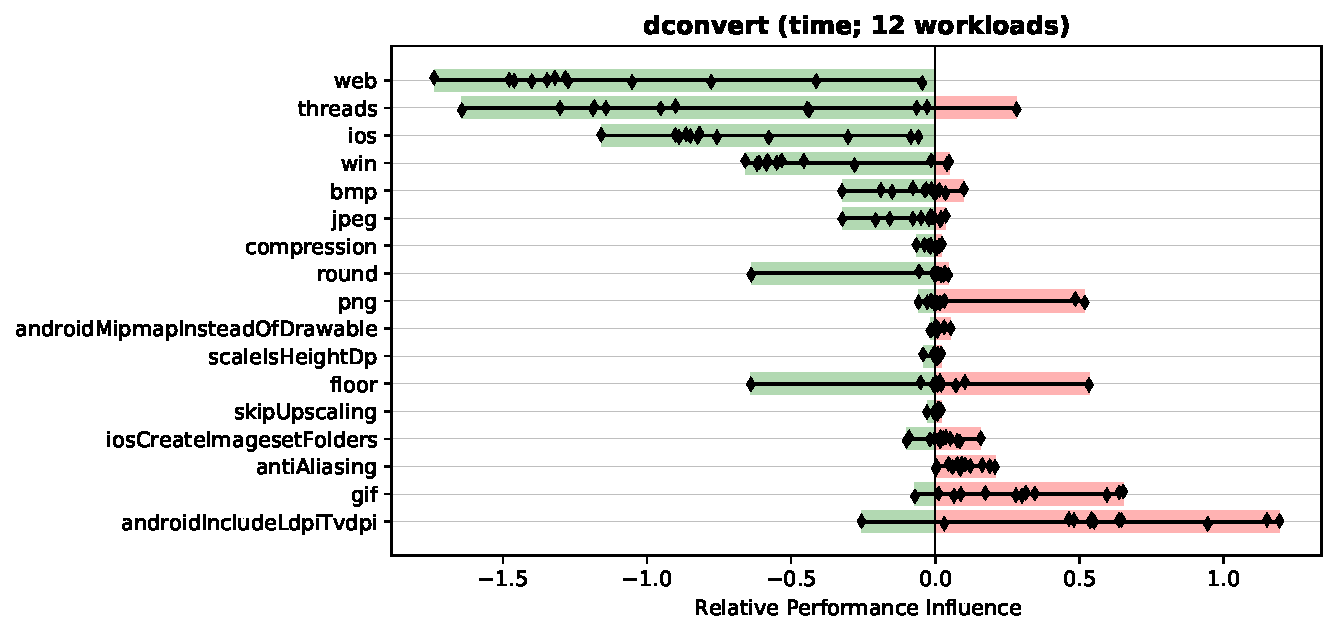
\includegraphics[width=\linewidth]{fse_22/dconvert_rq2.pdf}
	\end{subfigure}
	\begin{subfigure}{0.5\textwidth}
		\centering
		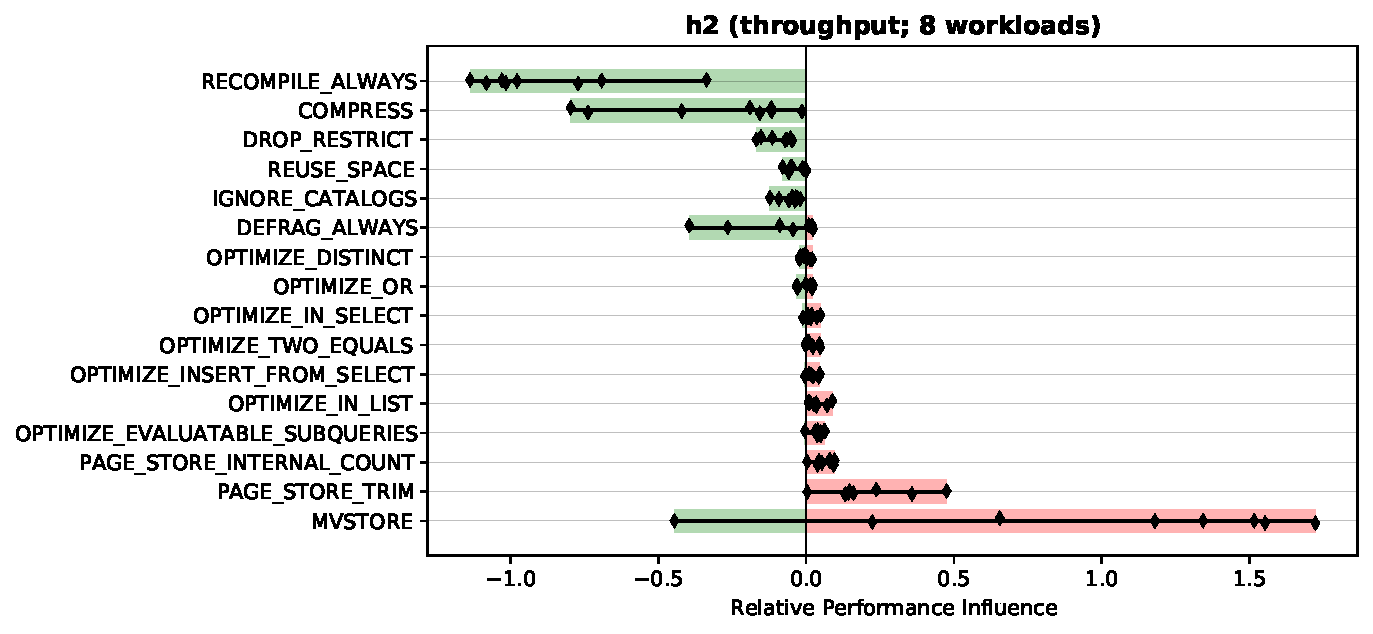
\includegraphics[width=\linewidth]{fse_22/h2_rq2.pdf}
	\end{subfigure}

	\begin{subfigure}{0.49\textwidth}
		\centering
		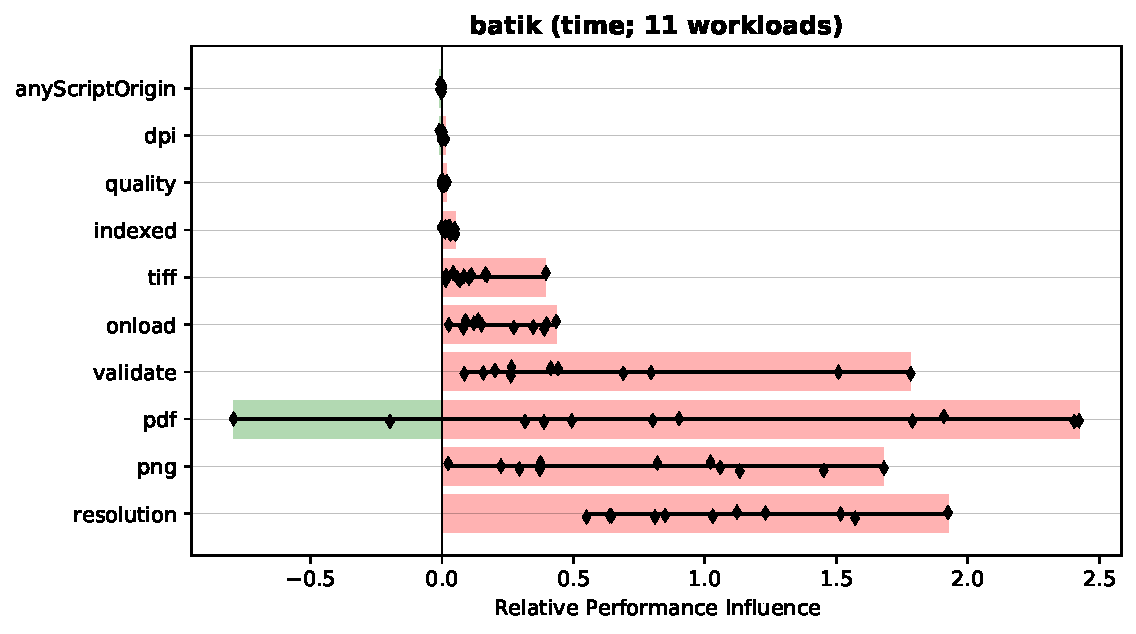
\includegraphics[width=0.8\linewidth]{fse_22/batik_rq2.pdf}
	\end{subfigure}
	\begin{subfigure}{0.5\textwidth}
		\centering
		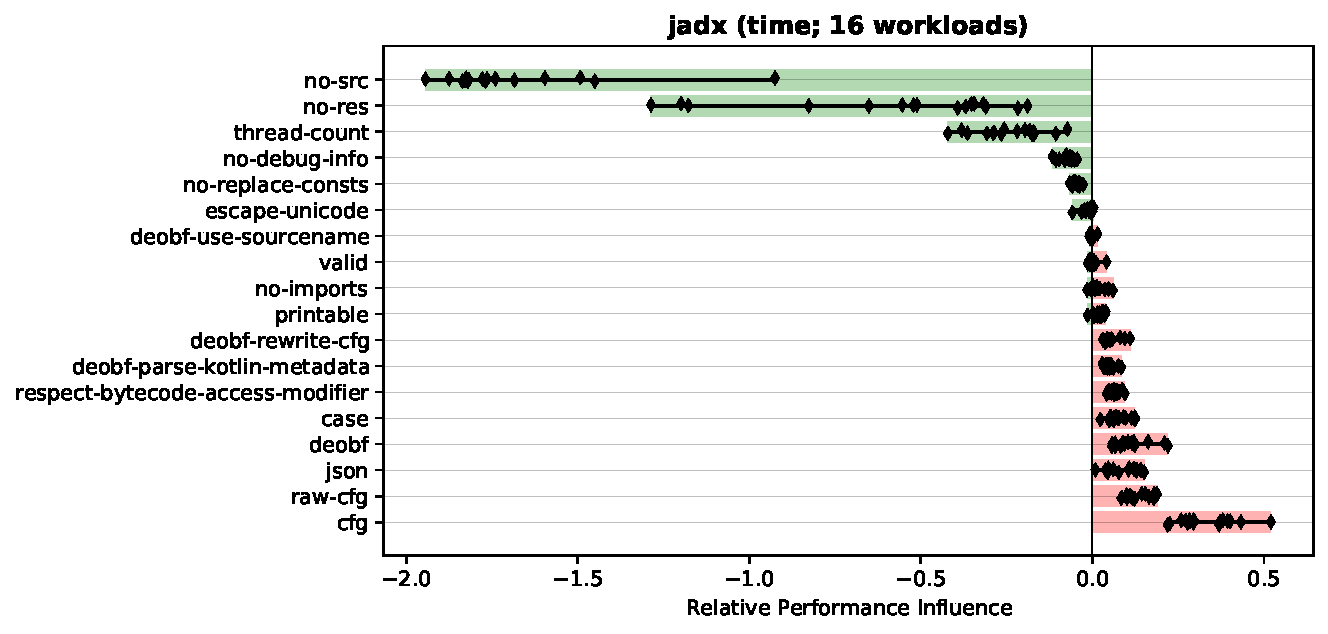
\includegraphics[width=\linewidth]{fse_22/jadx_rq2.pdf}
	\end{subfigure}
\caption{Relative performance influences (\textit{standardized regression coefficients}) for all configuration options across all workloads. Each black diamond ($\vardiamondsuit$) depicts a workload-specific performance influence. We highlight for each configuration option the effects with the highest \colorbox{red!20}{positive} and \colorbox{green!20}{negative} value. The line between the minimum and maximum performance influences denotes the overall range.}
\label{fig:results_influence}
\end{figure*}

{\color{black!40!white}\blindtext}
\vspace{2mm}
\greybox{\textbf{Summary} (\RQref{2}): \ldots}


\begin{comment}
We address this research question by learning and comparing performance models from the measurements of our experiments~\cite{dorn2020,siegmundPerformanceinfluenceModelsHighly2015,haDeepPerf2019,perfAL,guoVariabilityawarePerformancePrediction2013,sarkarCostEfficientSamplingPerformance,guo_2018_data,fourier_learning_2015,perLasso}. As a performance model effectively estimates the influence of individual configuration options on performance, we construct models not to predict unseen configurations but simply to explain differences observed in the performance distributions. So, for the construction of our performance models, we deliberately learn performance models using the entire sample set. 
To correct for multicollinearity~\cite{Daoud_2017} and to ensure that the obtained performance influences are interpretable, we drop several configuration options from the sample set, which has shown to be an effective practice~\cite{dorn2020}. For the training step, we exclude all mandatory configuration options since these by definition cannot contribute to performance variation. In addition, for each group of mutually exclusive configuration options, we discard one randomly selected group member.

Many different machine learning techniques have been used to obtain performance models, among others, based on linear regression~\cite{perLasso,siegmundPerformanceinfluenceModelsHighly2015,dorn2020}. To answer \RQref{2}, we learn a prediction model using multiple linear regression (least-squares method). We limit the set of independent variables to individual options rather than higher-order interactions to be consistent with the feature location used for \RQref{3} where we determine option-specific, but not interaction-specific code segments.

From the comparison of the performance model coefficients, we can answer \RQref{2} in detail and assess (1) how many configuration options, on average, change their influence, and (2) how many configuration options, in total, change their influence. For any pair of workload-specific performance models, we divide the performance model coefficients by the respective mean performance to make the model influences comparable across workloads. Henceforth, we will refer to these coefficients as \textit{relative performance influences.} Since these relative performance influences have been divided by the population mean, we report these without any unit.
\end{comment}
\begin{comment}
\begin{table}
	\footnotesize
	\centering
	\caption{Absolute number of configuration options whose relative performance influence changed by at least by threshold $t$ under, at least, one workload configuration.}
	\begin{tabular}{lr|rrrrr}
		\toprule
		& &  \multicolumn{5}{c}{\textbf{Difference threshold $t$}} \\
		\textbf{Software System} & \textbf{\#\,Opt.} & 0.01 &  0.05 &  0.1 &  0.2 &  0.5 \\
		\midrule
		\dconvert & 23 &    14 &    12 &    7 &    6 &    1 \\
		\jumper & 36 &   30 &    29 &   29 &   25 &    9 \\
		\batik &  20 &  10 &     7 &    6 &    6 &    5 \\
		\kanzi & 29 &   26 &    26 &   25 &   20 &    9 \\
		\jadx & 20 &   19 &     9 &    5 &    4 &    2 \\
		\htwo & 17 &   16 &     5 &    3 &    1 &    0 \\
		\bottomrule
	\end{tabular}
	\label{tab:total_changes}
\end{table}
\begin{table}
	\centering\footnotesize
	\caption{Average number of configuration options whose relative performance influence changed by, at least, by threshold $t$ across all workload combinations.}
	\begin{tabular}{lr|rrrrr}
		\toprule
		& & \multicolumn{5}{c}{\textbf{Difference threshold $t$}} \\
		\textbf{Software System} & \textbf{\#\,Opt.} & 0.01 &  0.05 &  0.1 &  0.2 &  0.5 \\
		\midrule
		\dconvert & 23 &  8.89 &  5.29 &  3.55 &  1.65 & 0.09 \\
		\jumper & 36 & 24.73 & 19.87 & 16.27 & 11.40 & 4.33 \\
		\batik & 20 &  7.22 &  4.47 &  3.62 &  2.95 & 1.18 \\
		\kanzi & 29 & 23.61 & 15.83 & 10.33 &  6.33 & 2.56 \\
		\jadx & 20 & 10.32 &  4.28 &  2.51 &  1.38 & 0.33 \\
		\htwo & 17 & 7.39 &  2.43 &  1.04 &  0.43 & 0.00 \\
		\bottomrule
	\end{tabular}
	\label{tab:average_changes}
\end{table}
\end{comment}



\clearpage
\section{Exploring Categories of Sensitivity}\label{sec:categories}

\subsection{Hypotheses}



\subsection{Code Coverage and Performance}\label{sec:rq3}
So far, we have only studied how different workloads can shape the overall performance and how they can affect the performance influence of configuration options. In addition, we want to know how the observed variation emerges from  varying the workload. To understand workload effects at a finer granularity, we travel back to the level of code and extend our perspective on the problem with statement coverage data. 

\paragraph*{Operationalization}
To approach this research question, we relate two types of variation for pairs of workloads. On the one hand, we compare the relative performance influences of an option. That is, we compute the absolute difference between the relative performance influences. On the other hand, we determine how much option-specific code (code segments that implement or regulate a functionality related to the configuration option) is covered under both workloads. That is, we ask how similar both workloads cover option-specific code. If the same part of option-specific code is executed under both workloads but we observe variation in the performance influence, this suggests that both workloads utilize the same code differently.



For each option and pair of workloads, in the following, we relate the difference in performance influence (performance influence variation) with the Jaccard similarity for option code (code coverage variation) for all pairs of workloads.

\subsubsection{Feature Location}
To reason about option-specific code, we require a mapping of configuration options to code. First, we obtain a baseline of \textit{all} option code within the scope of our entire workload selection. For each workload $w \in W$, we compute the set of code lines that depend on option $o \in O$. Let $C_{o}$ be the set of configurations with option $o$ selected, and $C_{\neg o}$ with option $o$ deselected. To obtain $S_{w, o}$, we follow a strategy similar to \textit{spectrum-based feature location}~\cite{michelon_spectrum_2021} and subtract the set of the code lines covered under $C_{\neg o}$ from those of $C_{o}$:

\begin{equation}%\todo{example from Figure~\ref{fig:intro}}
	S_{w, o} = \bigcup_{p \in C_{o}} S_{w}(p) ~ \setminus ~ \bigcup_{q \in C_{\neg o}} S_{w}(q)
\end{equation}

While $S_{w, o}$ yields an approximation of option-dependent code for a single workload, we then aggregate the approximations for each workload $w\in W$ to obtain the set of lines that depend on a configuration option $o$ and are executed in, at least, one workload,~$S_{o}$: 

\begin{equation}
	S_{o} = \bigcup_{w \in W} S_{w, o}
\end{equation}

While this aggregated set is not a ground truth, it enables us to reason about differences in option-dependent code within the scope of our selected workloads. That is, the expressiveness of this baseline depends on the diversity of the workloads in question. We discuss this limitation in Section~\ref{sec:construct_validity}. From the ratio of option-specific code per workload to option-specific code across workloads, $\mid S_{w_1, o}\mid/~{\mid S_{w_2, o}\mid}$, we can estimate the coverage of option-dependent code. By comparing the sets $S_{w_1, o}$ and $S_{w_2, o}$ for any two workloads $w_1$ and $w_2$, we can estimate similarity between the option-code coverage via the Jaccard set similarity index. We review further techniques for feature location in Section~\ref{sec:related}.

\paragraph*{Results}
{\color{red}\ldots}

\greybox{\textbf{Summary} (\RQref{3}):\ldots
}

\section{Discussion}\label{sec:discussion}

\subsection{Threats to Validity}
\subsubsection{Internal Validity}\label{sec:internal_validity}
Threats to \emph{internal validity} include measurement noise which may distort our classification into categories (Section~\ref{sec:rq1}) and model construction (Section~\ref{sec:rq2}). We mitigate this threat by repeating each experiment five times and reporting the median as a robust measure. For \htwo, we confirmed a negligible measurement variation in a separate pre-study.
Another potential threat is that the coverage analysis with \mbox{\textsc{JaCoCo}} entails a noticeable instrumentation overhead, which may distort performance observations. We mitigate this threat by separating the experiment runs for coverage assessment and performance measurement. In the case of \htwo, the load generator of the \textsc{OLTPBench} framework~\cite{difallah_oltp_2013} ran on the same machine as the database since we were testing an embedded scenario but thus introduced only negligible variation and overhead.

\subsubsection{External Validity}\label{sec:external_validity}
The selection of subject systems all written in Java poses a threat to \emph{external validity}. While our motivation for this selection is primarily practical (cf. Section~\ref{sec:setup}), we mitigate this threat by selecting subject systems from a variety of application domains (cf.~Table~\ref{tab:subject_systems}). Nonetheless, one cannot necessarily conclude that our results hold for other domains and programming languages. 

\subsubsection{Construct Validity}\label{sec:construct_validity}
Regarding \emph{construct validity}, the profiler \textsc{JaCoCo} instruments Java byte code instructions rather than statements, which leads to some minor imprecision when mapping covered instructions back to the original statements. Transitively, this also affects the precision of our feature location (cf. Section~\ref{sec:rq3}). This drawback, however, is not limited to this particular profiler but applies to most profilers operating on byte code. 
Superimposition in our feature location technique is sound, but, by design, incomplete, since no set of workloads is guaranteed to cover all feature code. We selected a variety of different workloads as a countermeasure, yet our study is exploratory. 

\subsection{Implications for Practitioners}

\begin{equation}
	\Pi(C) = {\color{blue}\underbrace{\beta_1 c_1}_{\text{Not input-sensitive}}} + {\color{green!40!black}\underbrace{\beta_2 c_2}_{\substack{\text{Scaling with}\\ \text{the workload}}} } + {\color{red!40!black}\underbrace{\beta_3 c_3}_{
			\substack{\text{vvv}\\\text{vvv}}	
	}} +\ldots \beta_0
\end{equation}

\subsection{Implications for Researchers}
\subsection{Future Work}
\section{Related Work}\label{sec:related}
\paragraph*{Feature Location}\label{sec:feature_location}
The problem of determining which code implements which functionality in a software system is known as \emph{feature location}~\cite{rubin_feature_2013}. Most feature location approaches either employ static or dynamic program analysis to infer a mapping between features and code. As for static analyses, variables that encode configuration options are tainted and, from tracing dataflow and controlflow, one can infer code sections tainted by such variables~\cite{velez_2020_configcrusher_jase,lillack_2018_lotrack_tse,luo_2019_cova}.
While static analyses can yield precise results, scalability is often limited by the exploration of all possible execution paths. To mitigate this shortcoming, dynamic taint analysis taints variables similarly to the static approaches, but only follows one execution path~\cite{bell_phosphor_2014,velez_comprex_2021,splat_kim_2013}. From few executions of different configurations, one can extract feature-specific code. 
Aside from program analysis, a more tame, but also less precise approach is to use code coverage information, such as execution traces.
The rationale is that by exercising feature code, for instance via enabling configuration options or running corresponding tests, its location can be inferred from code coverage differences. Applications of such an approach have been studied not only for feature location~\cite{wong_integrated_2005,sulir_annotation_2015,michelon_spectrum_2021,perez_framing_2016}, but root in program comprehension~\cite{wilde_early_1996,wilde_reconnaissance_1995,sherwood_reducing_nodate,perez_diagnosis_2014,castro_pangolin_2019} and fault localization~\cite{agrawal_fault_1995,wong_faultloc_2016}. 

\paragraph*{Workload-specific Performance}\label{sec:workload_performance}
In performance and load testing, it is a common practice to select a workload that is reflective of the software system in question~\cite{ceesay2020,papadopoulos2021}. This can be achieved by constructing workloads, among others, from usage patterns~\cite{calzarossa2016}, or by increasing the workload coverage by using a mix of different workloads rather than a single one~\cite{jiang2015survey}.
The benefit of using more than one specific workload for performance models is illustrated by the work of \citeauthor{liao_2020_using_emse}~\cite{liao_2020_using_emse}. For two different versions of a software system, they learn performance models based on disjoint sets of workloads. From the comparison of both performance models, they were able to identify performance shifts as the workload bias was averaged out.

\citeauthor{jamishidi_transfer_2017} observe that performance influences across different environments remain largely congruent and differences only affect small numbers of configuration options. Workload-specific differences can be learned efficiently via transfer learning~\cite{jamishidi_transfer_2017,jamshidi_transfer_gp_2017,ding_bayesian_2020}, where an existing workload-specific performance model is adapted to a new workload by explicitly learning a transfer function. \citeauthor{jamshidi_learning_2018} exploit similarities in performance behavior across workloads to guide the configuration sampling process an efficiently learn transfer functions~\cite{jamshidi_learning_2018}. {\color{purple} For software verification tools, \citeauthor{koc_satune_2021} incorporate program characteristics (e.g., the number of loops) as features orthogonal to configuration options into the problem space for performance modeling.}


\section{Summary}\label{sec:conclusion}


